\documentclass[11pt, twoside]{article}   	% use "amsart" instead of "article" for AMSLaTeX format
\usepackage{geometry}                		% See geometry.pdf to learn the layout options. There are lots.
\geometry{a4paper}                   		% ... or a4paper or a5paper or ... 
\linespread{1.0}
%\geometry{landscape}                		% Activate for rotated page geometry
%\usepackage[parfill]{parskip}    		% Activate to begin paragraphs with an empty line rather than an indent
\usepackage{graphicx}				% Use pdf, png, jpg, or eps§ with pdflatex; use eps in DVI mode
								% TeX will automatically convert eps --> pdf in pdflatex		

\pagestyle{headings}

%SetFonts

%\usepackage{mathrsfs}
\usepackage{amsthm, amsmath, amssymb}
%\usepackage{mathspec}

\usepackage{unicode-math}
%\usepackage{fourier}
%\usepackage{fontspec}
\setmathfont{STIX Two Math}
\setmathfont{STIX Two Math}[StylisticSet = 1, range = scr]
\setmathrm{STIX Two Math}
%\usepackage{newpxmath}
\setmainfont{Scala}
%\setmonofont{SF Mono}
\usepackage{xeCJK}
\usepackage{bbold}

\usepackage{graphicx}

\def\rcurs{{\mbox{$\resizebox{.16in}{.08in}{\includegraphics{ScriptR}}$}}}
\def\brcurs{{\mbox{$\resizebox{.16in}{.08in}{\includegraphics{BoldR}}$}}}
\def\hrcurs{{\mbox{$\hat \brcurs$}}}

\usepackage{color, xcolor}
\usepackage{ebezier}
\usepackage{tikz}
%\usepackage{circuitikz}
\usepackage{physics2}
\usephysicsmodule{ab, braket, bm-um.legacy, diagmat}

\usepackage[colorlinks,
linkcolor = blue,
anchorcolor = blue,
citecolor = blue,
urlcolor = blue]{hyperref}

\usepackage{multirow}
\usepackage{makecell}
\usepackage{booktabs}
\usepackage{wrapfig}
\usepackage{caption}
\usepackage{lastpage}

\usepackage{appendix}
\theoremstyle{plain}
\newtheorem{lemma}{Lemma}[section]
\newtheorem{theorem}[lemma]{Theorem}
\newtheorem{axiom}[lemma]{Axiom}
\newtheorem{corollary}[lemma]{Corollary}
\newtheorem{proposition}[lemma]{Proposition}
\theoremstyle{definition}
\newtheorem{definition}[lemma]{Definition}
\newtheorem{remark}{Remark}[section]
\newtheorem{example}[lemma]{Example}

\usepackage{syntonly}
%\syntaxonly

\usepackage{fancyhdr}
\pagestyle{fancy}
\fancyhf{}
\fancyhead[R]{黄远墨~~\textsf{2023141220092}}
\fancyhead[L]{Homework Nov 4th, 2024}
\fancyfoot[C]{\thepage/\pageref{LastPage}}
\renewcommand{\headrulewidth}{0.5pt}

%\renewcommand{\footrulewidth}{0.5pt}

\title{Homework}
\author{黄远墨~~\textsf{2023141220092}}
\date{}							% Activate to display a given date or no date

\begin{document}
	% generates the title
	%\maketitle
	\thispagestyle{fancy}
	\section{Problem 5}
	\begin{description}
		\item[5.3] $\dfrac{2\lambda}{d} \times 50 \mathrm{cm} = 1 \mathrm{cm} \quad \Rightarrow
			\quad d = 63 \mu\mathrm{m}$.
		\item[5.4] $D = 2 \times \dfrac{1.22\lambda}{d} \times 3.76 \times 10^{8} \mathrm{m}, \quad
			\lambda = 632.8 \mathrm{nm}$.
			\begin{table}[htbp]
				\caption{Diameters}
				\centering
				\begin{tabular}{cc}
					\toprule
					on Earth $d$ & on Moon $D$\\
					\midrule
					$2 \mathrm{mm}$ & $290.3 \mathrm{km}$\\
					$2 \mathrm{m}$	& $290.3 \mathrm{m}$\\
					$5 \mathrm{m}$	& $116.1 \mathrm{m}$\\
					\bottomrule
				\end{tabular}
			\end{table}
		\item[5.6] $\theta_0 = 1.22 \lambda / D = 1.342 \times 10^{-7} \mathrm{rad} = 0.02768''$.
			The angular limit of resolution of a human eye is $1'$, $1' / 0.02768'' = 2167$.
		\item[5.9] \textbf{(1)} $\delta y = 0.61\lambda / 0.85 = 287 \mathrm{nm}$. \textbf{(2)}
			$\delta y = 0.61 \lambda / 1.45 = 168 \mathrm{nm}$, the limit of resolution of a human
			eye is $\delta y' = 25\mathrm{cm} \times 1' = 72.7\mu\mathrm{m}$. $\delta y' / \delta y
			= 432$.
		\item[5.13] $\theta = 2\lambda / d$, thus $\delta \theta = 2 \delta \lambda / d = 5 \times
			10^{-6} \mathrm{rad} = 1.03''$. While half the linewidth is $\Delta \theta \approx
			\frac{\lambda}{Nd} = 5 \times 10^{-6} \mathrm{rad} \sim \delta \theta$. 恰能分辨.
		\item[5.16] Let
			\begin{equation}
				s(x) = \sum_{n=-N}^{N - 1} \delta(x - 6 a (n + 1/2)), \quad
				t(x) =
				\begin{cases}
					1, & x \leq a/2,\\
					0, & \text{otherwise}.
				\end{cases}
			\end{equation}
			Their Fourier transformations
			\begin{align}
				\mathscr F\{s\} &:= \int_{-\infty}^\infty s(x) \mathrm e^{\mathrm{i}k x \sin\theta}
				\mathrm{d} x = \sum_{n = -N}^{N - 1} \mathrm e^{\mathrm{i}6ak\sin\theta (n + 1/2)} =
				\frac{\sin 6Nak\sin\theta}{\sin 3ak\sin\theta},\\
				\mathscr F\{t\} &:= \int_{-\infty}^\infty t(x) \mathrm e^{\mathrm{i}k x \sin\theta}
				\mathrm{d} x = \left. \frac{\mathrm e^{\mathrm{i}k x \sin\theta}}{\mathrm{i}k \sin
				\theta} \right|_{-a/2}^{a/2} = a \frac{\sin\frac{1}{2} k a \sin\theta}{\frac{1}{2}
				k a \sin\theta}.
			\end{align}
			If we define convolution $*: \mathbb R^{\mathbb R} \times \mathbb R^{\mathbb R} \to
			\mathbb R^{\mathbb R}$ as follows:
			\begin{equation}
				(f * g)(x) = \int_{-\infty}^\infty f(t) g(x-t) \mathrm{d} t,
			\end{equation}
			it is well-know that $\mathscr F$ is an isomorphism: $\mathscr F\{f * g\} =
			\mathscr F\{f\} \cdot \mathscr F\{g\}$.

			For \textbf{(1)} even numbered slits are blocked, and \textbf{(2)} odd numbered slits
			are blocked, both of their aperature functions are $s * t$. Then the field distribution
			is
			\begin{equation}
				E(\theta) = \frac{E_0}{a} \mathscr F\{s * t\} = \frac{E_0}{a} \mathscr F\{s\} \cdot
				\mathscr F\{t\} = E_0 \left( \frac{\sin 12N\alpha}{\sin 6\alpha} \right)
				\left( \frac{\sin\alpha}{\alpha} \right),
			\end{equation}
			where $\alpha = \frac{1}{2}k a \sin\theta$. Intensity distribution
			\begin{equation}
				I(\theta) = \frac{I_0}{E_0^2} \ab|E(\theta)|^2 = I_0 \left( \frac{\sin12N\alpha}{
				\sin6N\alpha} \right)^2 \left( \frac{\sin\alpha}{\alpha} \right)^2.
			\end{equation}

			\textbf{(3)} The aperature function is $(s(x) + s(x - 2a)) * t$. By calculation:
			\begin{equation}
				\mathscr F\{s(x) + s(x - 2a)\} = 2 \mathrm e^{2\mathrm{i}\alpha} \cos2\alpha \cdot
				\mathscr F\{s\}.
			\end{equation}
			Therefore the field distribution is
			\begin{equation}
				E(\theta) = \frac{E_0}{a} \mathscr F\{(s(x) + s(x - 2a)) * t\} = 2 E_0 \mathrm e^{2
				\mathrm{i}\alpha} \cos2\alpha \left( \frac{\sin 12N\alpha}{\sin 6\alpha} \right)
				\left( \frac{\sin\alpha}{\alpha} \right),
			\end{equation}
			and intensity distribution
			\begin{equation}
				I(\theta) = \frac{I_0}{E_0^2} \ab|E(\theta)|^2 = 4 I_0 \cos^2 2\alpha \left( \frac{
				\sin12N\alpha}{\sin6N\alpha} \right)^2 \left( \frac{\sin\alpha}{\alpha} \right)^2.
			\end{equation}

		\item[5.18] According to Fresnel-Kirchhoff formula,
			\begin{equation}
				E = -\frac{\mathrm{i}E_0}{\lambda} \int_L^{\sqrt{L^2 + (D/2)^2}}2\pi r \mathrm{d} r
				\frac{
				\mathrm e^{\mathrm{i} k r}}{r} \frac{1 + L/r}{2} = -\mathrm{i}\pi \frac{E_0}{\lambda}
				\int_L^{\sqrt{L^2 + (D/2)^2}} \left( 1 + \frac{L}{r} \right) \mathrm e^{\mathrm{i}
				k r} \mathrm{d} r,
			\end{equation}
			where $L = 1.5 \mathrm{m}$, $D = 2.6 \mathrm{mm}$ and $\lambda = 589 \mathrm{nm}$. Since
			$D \ll L$, we have $L/r \approx 1$, and thus
			\begin{equation}
				E \approx -\mathrm{i}k E_0 \int_L^{\sqrt{L^2 + (D/2)^2}}
				\mathrm e^{\mathrm{i} k r} \mathrm{d} r = 2 E_0 \mathrm e^{\mathrm{i} \delta} \sin
				\frac{\pi}{\lambda} \left( \sqrt{L^2 + (D/2)^2} - L \right),
			\end{equation}
			where $\delta = -\frac{\pi}{2} + \frac{k}{2} \left( L + \sqrt{L^2 + (D/2)^2} \right)$.
			That is
			\begin{equation}
				I = \frac{I_0}{E_0^2} \ab|E|^2 \approx 4 I_0 \sin^2 \frac{\pi D^2}{8\lambda L}
				= 4 I_0 \times 0.14.
			\end{equation}
			Then center point is \textbf{dark}.

			To make the center point bright, let $\frac{\pi D^2}{8 \lambda L} = (2n + 1)
			\frac{\pi}{2}$, only for small $n \in \mathbb N$,
			\begin{equation}
				\begin{aligned}
					D &= \sqrt{4\lambda L (2n + 1)} = \sqrt{2n + 1} \times 1.88\mathrm{mm}\\
					  &= 1.88\mathrm{mm},~3.26\mathrm{mm},~4.20\mathrm{mm},~4.97\mathrm{mm},...
				\end{aligned}
			\end{equation}
		\item[5.22] Using the result obtained in \textbf{5.18},
			\begin{equation}
				\begin{aligned}
					E &\approx -E_0 \left[ \mathrm e^{\mathrm{i}k\sqrt{L^2 + r_2^2}} - \mathrm e^{
					\mathrm{i}kL} + \frac{1}{4} \mathrm e^{\mathrm{i}k\sqrt{L^2 + r_1^2}}
					- \frac{1}{4} \mathrm e^{\mathrm{i}k\sqrt{L^2 + r_2^2}} \right]\\
					  &\approx -E_0 \mathrm e^{\mathrm{i}kL} \left[ \left( \mathrm e^{\mathrm{i}k
					  r_2^2/(2L)} - 1 \right) + \frac{1}{4} \left( \mathrm e^{\mathrm{i}k r_1^2/(2L)}
					  - \mathrm e^{\mathrm{i}k r_2^2/(2L)} \right) \right]\\
					  &= -2 E_0 \left( 1 + \frac{1}{4} \mathrm e^{\mathrm{i}\delta} \right)
					  \mathrm e^{\mathrm{i}(\delta / 2 + kL)} \sin \frac{\delta}{2}, \quad \delta =
					  \frac{k r_2^2}{2L} = \pi, \quad \text{using $r_1^2 = 2 r_1^2$},\\
					  &= -\mathrm{i}\frac{3}{2} E_0 \mathrm e^{\mathrm{i}kL}
					  = -\frac{3\mathrm{i}}{2}E_0,
				\end{aligned}
			\end{equation}
			where $E_0$ is the amplitude on the aperature. Then the intensity is
			\begin{equation}
				I = \frac{I_0}{E_0^2}\ab|E|^2 = \frac{9}{4} I_0.
			\end{equation}
		\item[5.23] \textbf{(1)} $\frac{2\pi}{\lambda} \left( \sqrt{L^2 + r_4^2} - L \right) = \pi +
			3 \times 2\pi \quad \Rightarrow \quad r_4 \approx \sqrt{7\lambda L} = 5.916\mathrm{mm}$.

			\textbf{(2)} $\frac{1}{10\mathrm{m}} = \frac{(2n-1)\lambda}{r_n^2} = \frac{1}{2\mathrm{m}
			} + \frac{1}{s} \quad \Rightarrow \quad s = -2.5\mathrm{m}$, that is, $S$ is imaged
			$2.5\mathrm{m}$ from the Fresnel zone plate, and on the same side of $S$.
	\end{description}

	\section{Simulation}

	Applying the same method in \textbf{Problem~5.16}, we have
	\begin{align}
		&I_{\text{Diffraction}}(\theta) = \left( \frac{\sin\alpha}{\alpha} \right)^2,\\
		&I_{\text{Interference}}(\theta) = \left( \frac{1}{N} \frac{\sin N\beta}{\sin\beta}
		\right)^2,\\
		&I(\theta) = I_0 \cdot I_{\text{Diffraction}}(\theta) \cdot I_{\text{Interference}}(\theta),
	\end{align}
	where $\alpha = \frac{1}{2} k a \sin\theta$ and $\beta = \frac{1}{2} k d \sin\theta$.
	$I_{\text{Diffraction}}(\theta)$ and $I_{\text{Interference}}(\theta)$ are dimensionless and
	normalized so that their maxima are $1$.

	\begin{figure}[htbp]
		\centering
		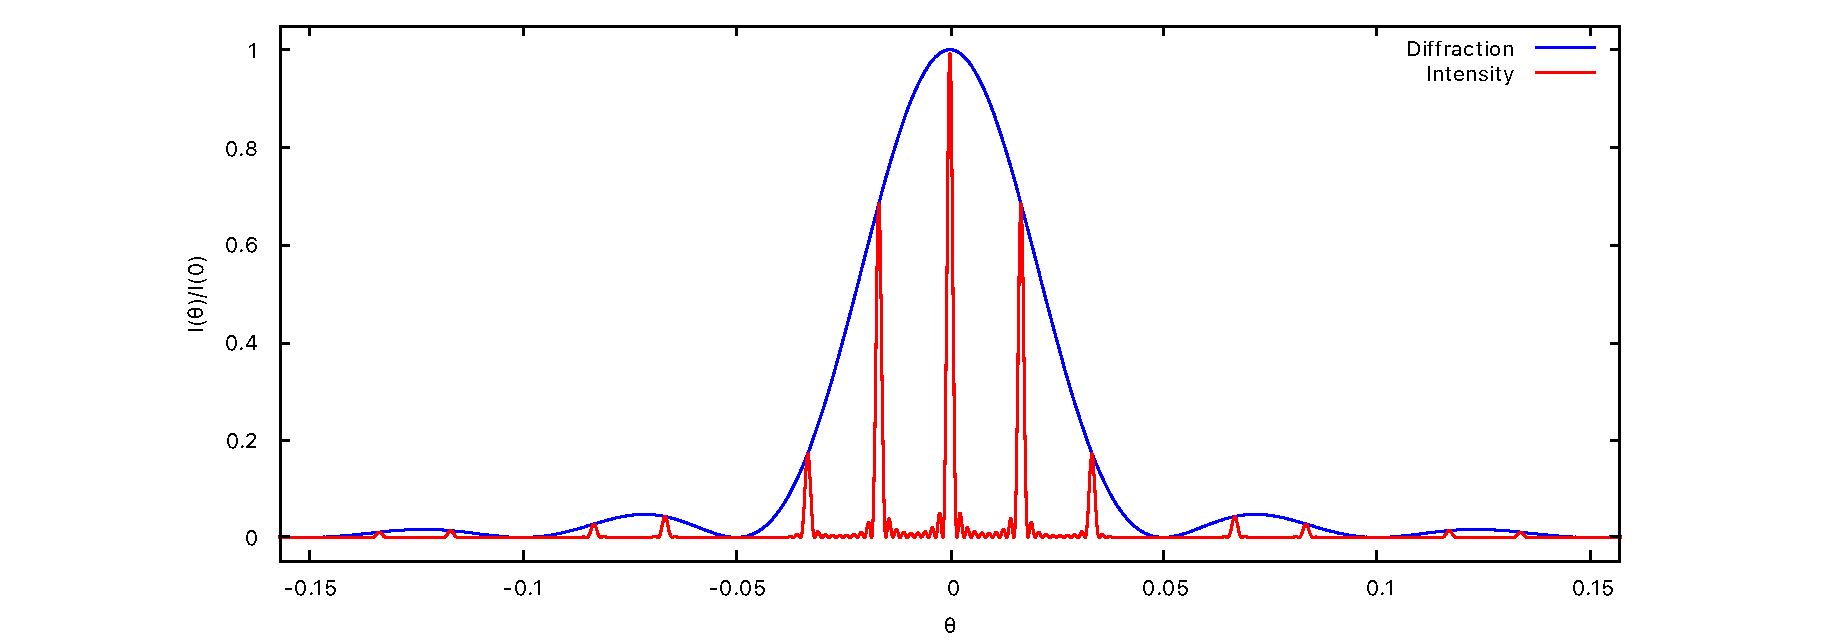
\includegraphics[width=\linewidth]{DiffractionFactor}
		\captionsetup{font={footnotesize}}
		\caption{$\lambda = 500\mathrm{nm}, N = 10, d = 30\mu\mathrm{m}, a = 10\mu\mathrm{m}$}
	\end{figure}
	
	\begin{description}
		\item[(1)] We can see in Figure 1 that the intensity $I(\theta)$ is enveloped by the
			diffraction factor $I_{\text{Diffraction}}(\theta)$. Thus the position of the
			principal maxima is determined by the interference factor $I_{\text{Interference}}(
			\theta)$, while their intensities are controlled by the diffraction factor.
		\item[(2)] Diffraction figures of different $N$ are ploted in Figure 2-4 ($\lambda = 500
			\mathrm{nm}, d = 20\mu\mathrm{m}, a = 7\mu\mathrm{m}$). As $N$ increases, the width of
			the principal maxima narrows.
		\item[(3)] Diffraction figures of different $d$ are ploted in Figure 5-7 ($\lambda = 500
			\mathrm{nm}, N = 10, a = 7\mu\mathrm{m}$). As $d$ increases, the distance between two
			nearest principal maxima narrows and roughly proportional to $1/d$.
		\item[(4)] Diffraction figures of different $a$ are ploted in Figure 8-10 ($\lambda = 500
			\mathrm{nm}, N = 10, d = 20\mu\mathrm{m}$). As $d$ increases, the distance between two
			nearest interference minima narrows and roughly proportional to $1/a$.

	\begin{figure}[htbp]
		\begin{minipage}[t]{0.33\linewidth}
		\centering
		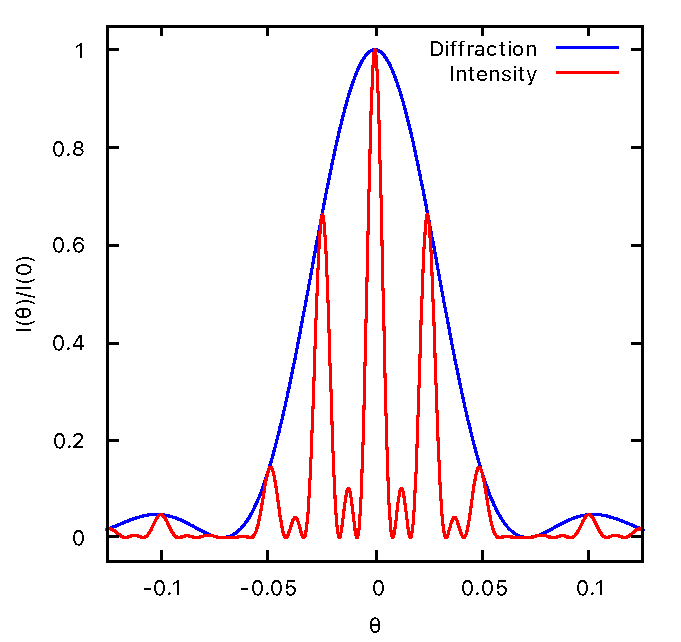
\includegraphics[width=0.9\linewidth]{N=3}
		\captionsetup{font={footnotesize}}
		\caption{$N=3$}
		\end{minipage}
		\begin{minipage}[t]{0.33\linewidth}
		\centering
		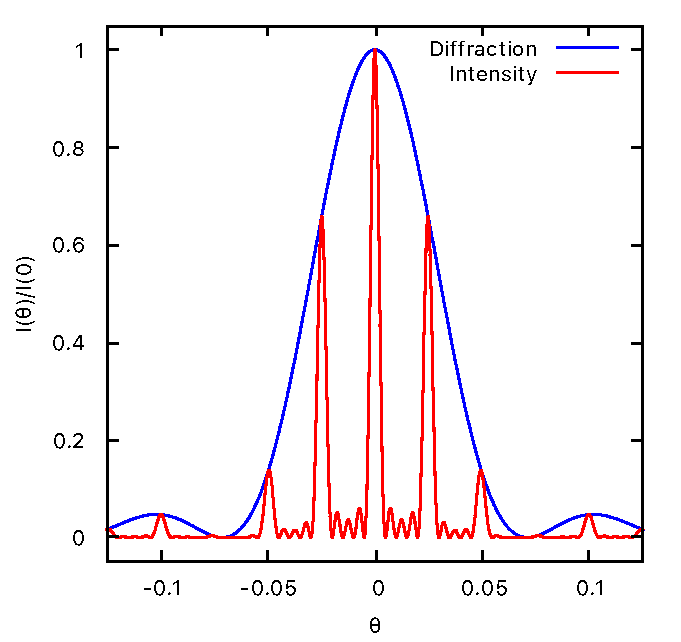
\includegraphics[width=0.9\linewidth]{N=5}
		\captionsetup{font={footnotesize}}
		\caption{$N=5$}
		\end{minipage}
		\begin{minipage}[t]{0.33\linewidth}
		\centering
		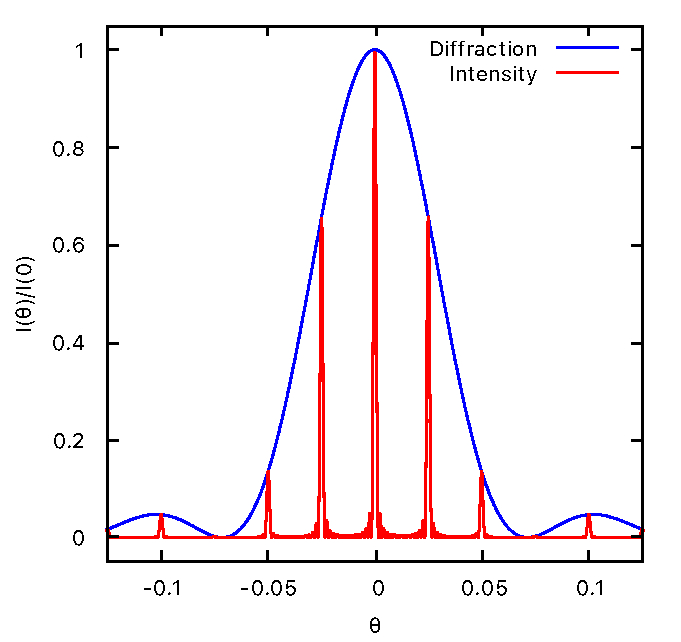
\includegraphics[width=0.9\linewidth]{N=15}
		\captionsetup{font={footnotesize}}
		\caption{$N=15$}
		\end{minipage}
		\medskip

		\begin{minipage}[t]{0.33\linewidth}
		\centering
		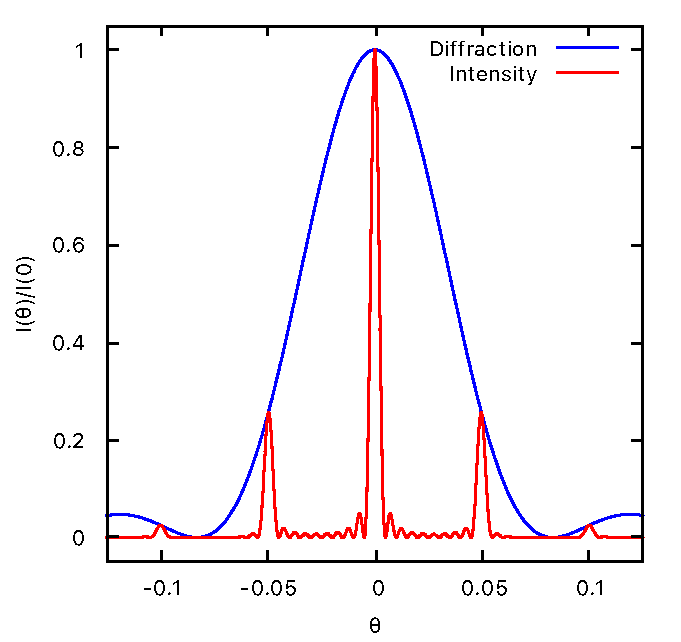
\includegraphics[width=0.9\linewidth]{d=10}
		\captionsetup{font={footnotesize}}
		\caption{$d=10\mu\mathrm{m}$}
		\end{minipage}
		\begin{minipage}[t]{0.33\linewidth}
		\centering
		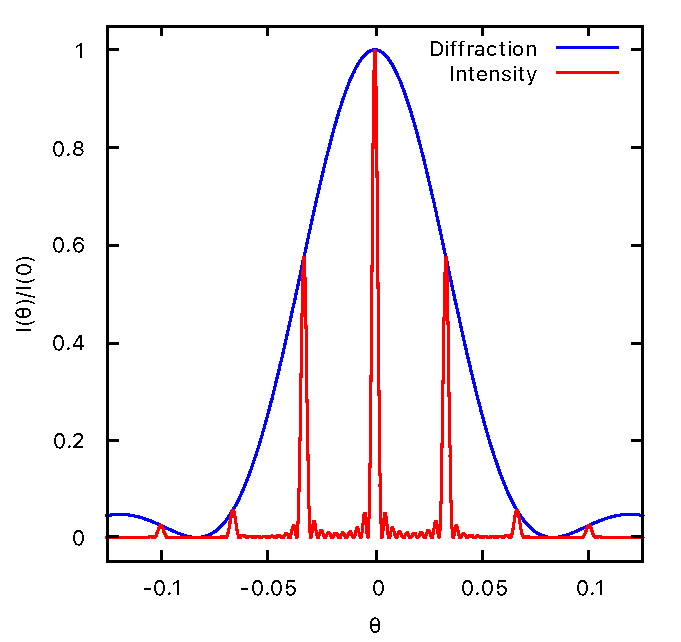
\includegraphics[width=0.9\linewidth]{d=15}
		\captionsetup{font={footnotesize}}
		\caption{$d=15\mu\mathrm{m}$}
		\end{minipage}
		\begin{minipage}[t]{0.33\linewidth}
		\centering
		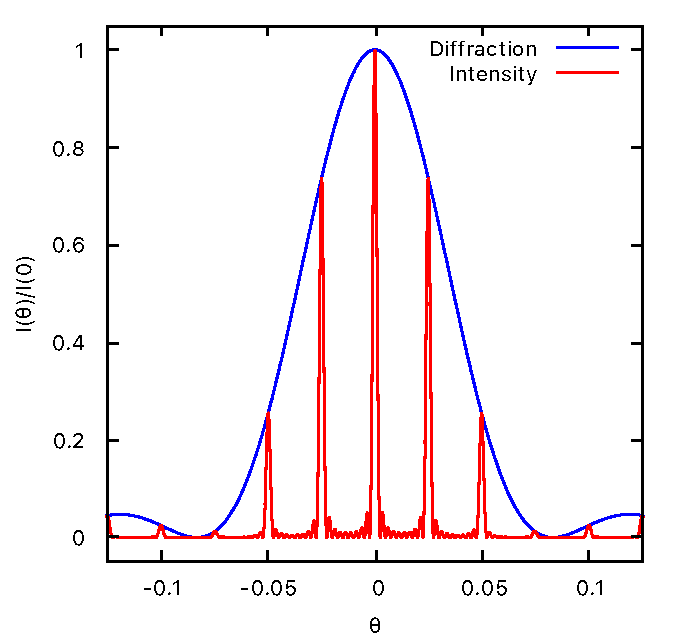
\includegraphics[width=0.9\linewidth]{d=20}
		\captionsetup{font={footnotesize}}
		\caption{$d=20\mu\mathrm{m}$}
		\end{minipage}
		\medskip

		\begin{minipage}[t]{0.33\linewidth}
		\centering
		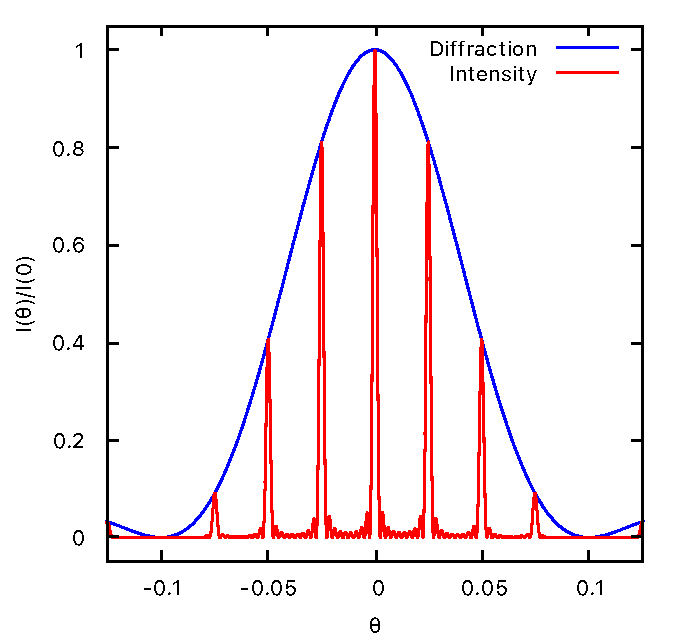
\includegraphics[width=0.9\linewidth]{a=5}
		\captionsetup{font={footnotesize}}
		\caption{$a=5\mu\mathrm{m}$}
		\end{minipage}
		\begin{minipage}[t]{0.33\linewidth}
		\centering
		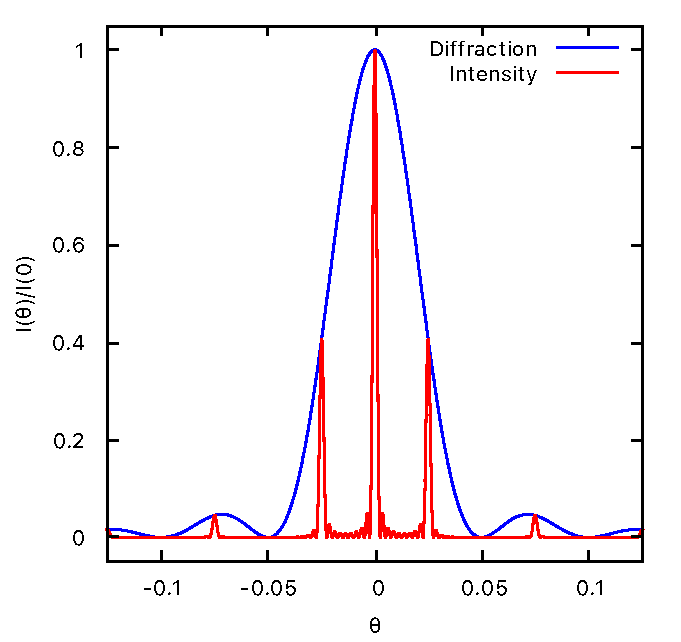
\includegraphics[width=0.9\linewidth]{a=10}
		\captionsetup{font={footnotesize}}
		\caption{$a=10\mu\mathrm{m}$}
		\end{minipage}
		\begin{minipage}[t]{0.33\linewidth}
		\centering
		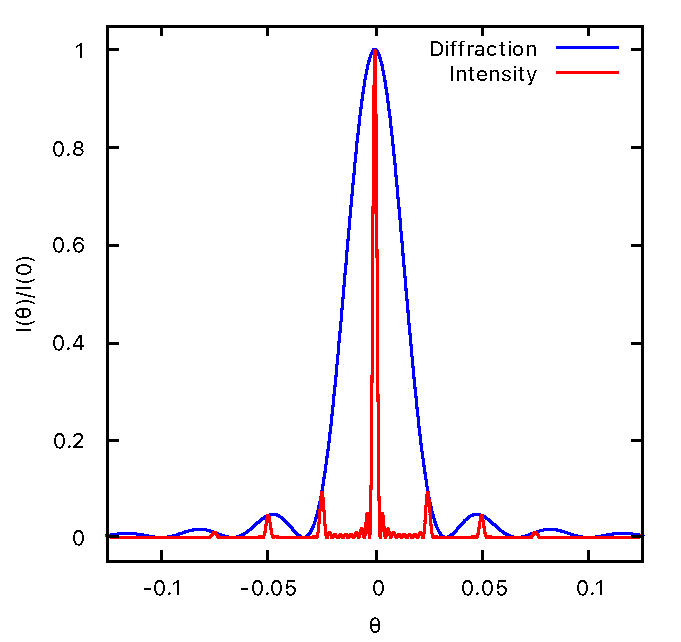
\includegraphics[width=0.9\linewidth]{a=15}
		\captionsetup{font={footnotesize}}
		\caption{$a=15\mu\mathrm{m}$}
		\end{minipage}
	\end{figure}

		\item[(5)] A missing order means an overlap of the maximum of interference factor and the
			minimum of diffraction factor. The missing orders are $\pm \left( d \cdot \mathrm{lcm}
			\left( \frac{1}{a}, \frac{1}{d} \right) \right) \mathbb N^+$, where $\mathrm{lcm}$
			denotes the least common multiple.

	\begin{figure}[htbp]
		\begin{minipage}[t]{0.33\linewidth}
		\centering
		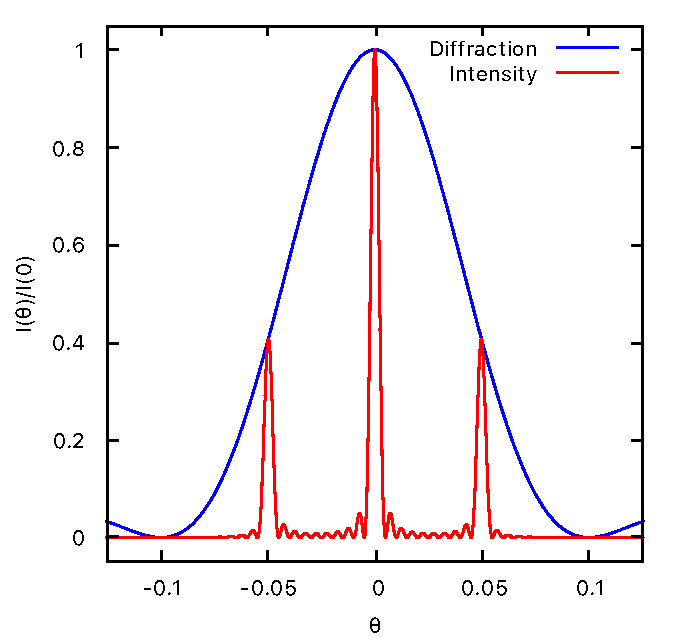
\includegraphics[width=0.9\linewidth]{5-10}
		\captionsetup{font={footnotesize}}
		\caption{\centering $a = 5\mu\mathrm{m}, d = 10\mu\mathrm{m}$
			\newline orders $\pm 2\mathbb N^+$ missed.}
		\end{minipage}
		\begin{minipage}[t]{0.33\linewidth}
		\centering
		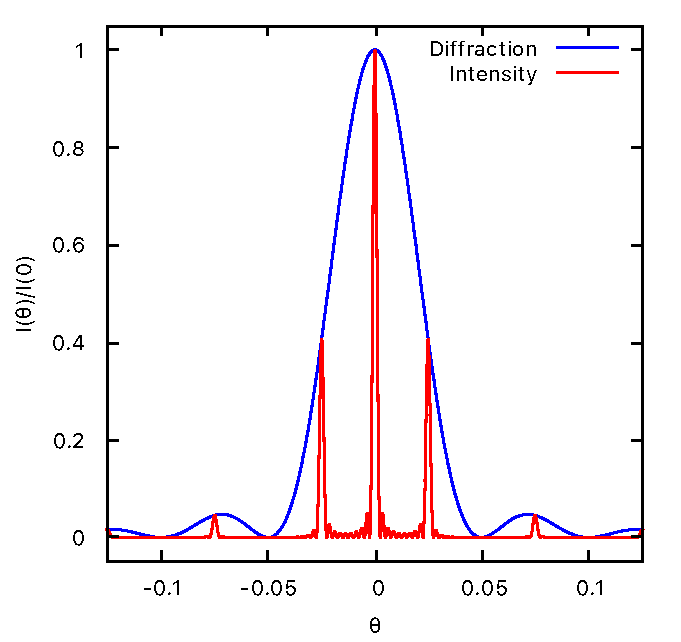
\includegraphics[width=0.9\linewidth]{10-20}
		\captionsetup{font={footnotesize}}
		\caption{\centering $a = 10\mu\mathrm{m}, d = 20\mu\mathrm{m}$
			\newline orders $\pm 2\mathbb N^+$ missed.}
		\end{minipage}
		\begin{minipage}[t]{0.33\linewidth}
		\centering
		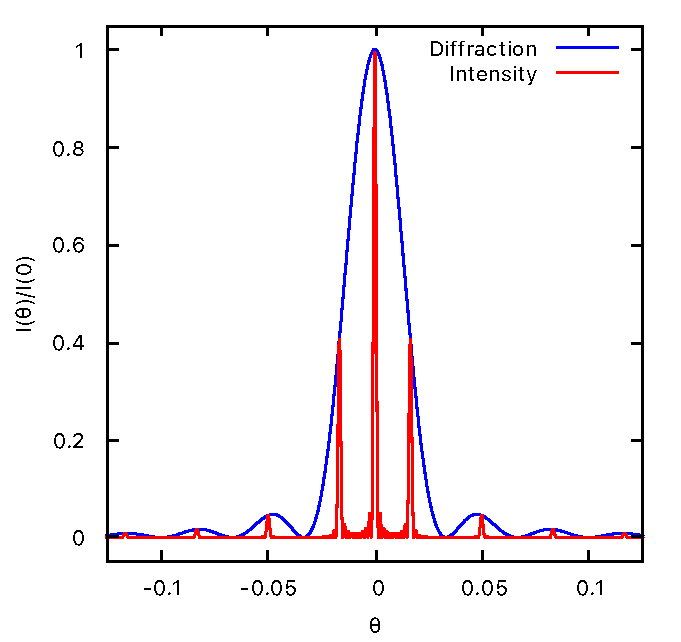
\includegraphics[width=0.9\linewidth]{15-30}
		\captionsetup{font={footnotesize}}
		\caption{\centering $a = 15\mu\mathrm{m}, d = 30\mu\mathrm{m}$
			\newline orders $\pm 2\mathbb N^+$ missed.}
		\end{minipage}
		\medskip

		\begin{minipage}[t]{0.33\linewidth}
		\centering
		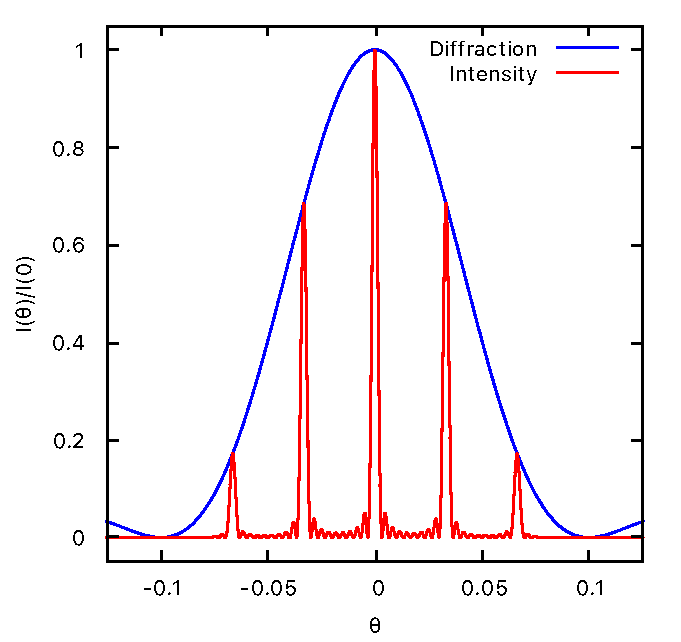
\includegraphics[width=0.9\linewidth]{5-15}
		\captionsetup{font={footnotesize}}
		\caption{\centering $a = 5\mu\mathrm{m}, d = 15\mu\mathrm{m}$
			\newline orders $\pm 3\mathbb N^+$ missed.}
		\end{minipage}
		\begin{minipage}[t]{0.33\linewidth}
		\centering
		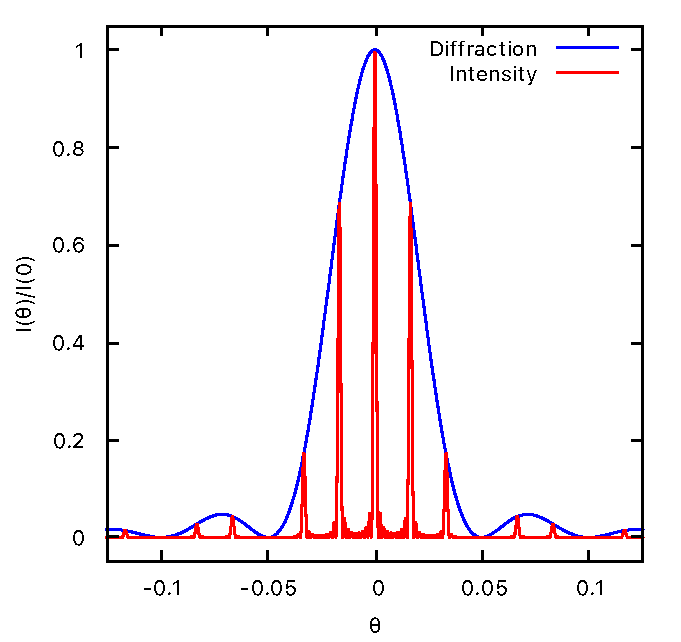
\includegraphics[width=0.9\linewidth]{10-30}
		\captionsetup{font={footnotesize}}
		\caption{\centering $a = 10\mu\mathrm{m}, d = 30\mu\mathrm{m}$
			\newline orders $\pm 3\mathbb N^+$ missed.}
		\end{minipage}
		\begin{minipage}[t]{0.33\linewidth}
		\centering
		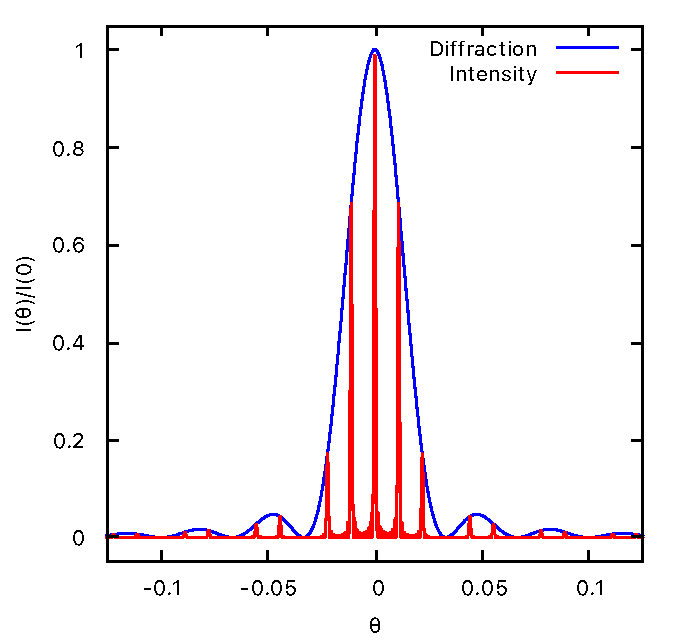
\includegraphics[width=0.9\linewidth]{15-45}
		\captionsetup{font={footnotesize}}
		\caption{\centering $a = 15\mu\mathrm{m}, d = 45\mu\mathrm{m}$
			\newline orders $\pm 3\mathbb N^+$ missed.}
		\end{minipage}
		\medskip

		\begin{minipage}[t]{0.33\linewidth}
		\centering
		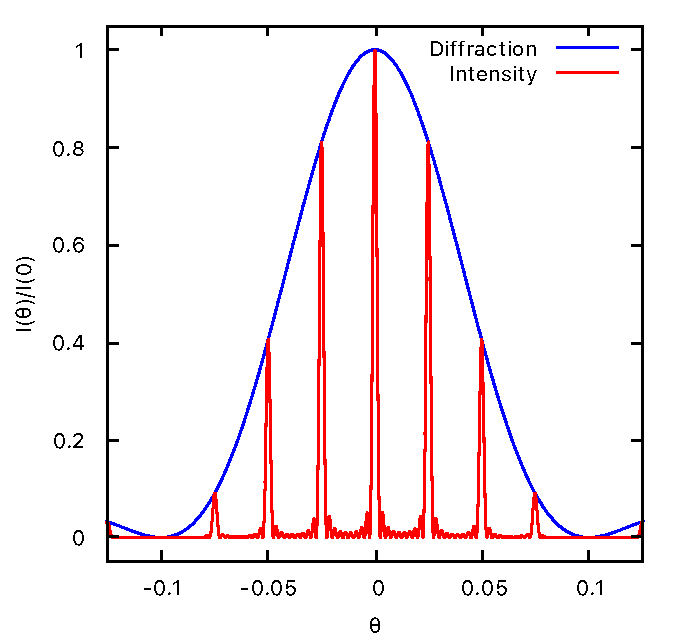
\includegraphics[width=0.9\linewidth]{5-20}
		\captionsetup{font={footnotesize}}
		\caption{\centering $a = 5\mu\mathrm{m}, d = 20\mu\mathrm{m}$
			\newline orders $\pm 4\mathbb N^+$ missed.}
		\end{minipage}
		\begin{minipage}[t]{0.33\linewidth}
		\centering
		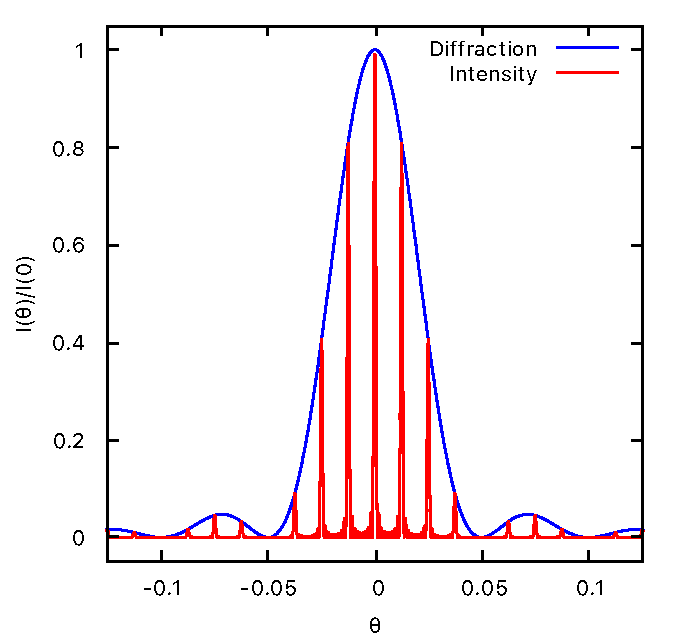
\includegraphics[width=0.9\linewidth]{10-40}
		\captionsetup{font={footnotesize}}
		\caption{\centering $a = 10\mu\mathrm{m}, d = 40\mu\mathrm{m}$
			\newline orders $\pm 4\mathbb N^+$ missed.}
		\end{minipage}
		\begin{minipage}[t]{0.33\linewidth}
		\centering
		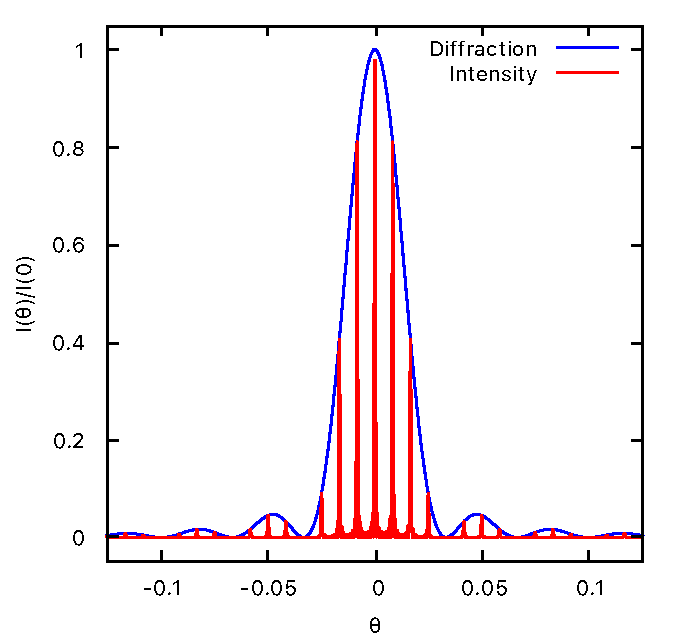
\includegraphics[width=0.9\linewidth]{15-60}
		\captionsetup{font={footnotesize}}
		\caption{\centering $a = 15\mu\mathrm{m}, d = 60\mu\mathrm{m}$
			\newline orders $\pm 4\mathbb N^+$ missed.}
		\end{minipage}
	\end{figure}
	\end{description}

\end{document}


